

 \begin{appendices}
 \newpage
 \section{Supporting data for experiments} \label{app: exp_data1}

 \begin{table}[!ht]
	\centering
	%
	\scriptsize
	\caption{Results of \tool, across compilers (\texttt{gcc} and \texttt{clang}) with different code optimization levels\\}\label{tab:diff_comp} %(O0, O2 and O3)

\begin{tabular}{ | p{2.28cm} | p{0.57cm} | p{0.57cm} | p{0.57cm} | p{0.57cm} | p{0.57cm} | p{0.57cm} | }
\hline
	. & Rank 1 & Top 5 & Top 10 & Tot. Sig. Func & Tot. Tar. func & Time (s)  \  \\ \hline
	clang\_O0-clang\_O2 & 0.193 & 0.525 & 0.911 & 15740 & 10141 & 262.4 \\ \hline
	clang\_O0-clang\_O3 & 0.194 & 0.517 & 0.91 & 15740 & 10100 & 208.9 \\ \hline
	clang\_O0-gcc\_O0 & 0.149 & 0.462 & 0.897 & 15740 & 14807 & 308.9 \\ \hline
	clang\_O0-gcc\_O2 & 0.241 & 0.509 & 0.872 & 15740 & 10579 & 206.3 \\ \hline
	clang\_O0-gcc\_O3 & 0.222 & 0.599 & 0.909 & 15740 & 10337 & 252.2 \\ \hline
	clang\_O2-clang\_O0 & 0.299 & 0.716 & 0.934 & 10141 & 15740 & 198.9 \\ \hline
	clang\_O2-clang\_O3 & 0.997 & 0.999 & 1 & 10141 & 10100 & 118.7 \\ \hline
	clang\_O2-gcc\_O0 & 0.2 & 0.651 & 0.925 & 10141 & 14807 & 212.9 \\ \hline
	clang\_O2-gcc\_O2 & 0.417 & 0.642 & 0.931 & 10141 & 10579 & 218.4 \\ \hline
	clang\_O2-gcc\_O3 & 0.511 & 0.92 & 0.983 & 10141 & 10337 & 232.6 \\ \hline
	clang\_O3-clang\_O0 & 0.298 & 0.71 & 0.929 & 10100 & 15740 & 244.2 \\ \hline
	clang\_O3-clang\_O2 & 0.99 & 0.997 & 0.998 & 10100 & 10141 & 136.2 \\ \hline
	clang\_O3-gcc\_O0 & 0.2 & 0.646 & 0.92 & 10100 & 14807 & 263.7 \\ \hline
	clang\_O3-gcc\_O2 & 0.414 & 0.638 & 0.928 & 10100 & 10579 & 183.3 \\ \hline
	clang\_O3-gcc\_O3 & 0.512 & 0.92 & 0.983 & 10100 & 10337 & 232.8 \\ \hline
	gcc\_O0-clang\_O0 & 0.419 & 0.897 & 0.981 & 14807 & 15740 & 423.5 \\ \hline
	gcc\_O0-clang\_O2 & 0.234 & 0.701 & 0.965 & 14807 & 10141 & 198.5 \\ \hline
	gcc\_O0-clang\_O3 & 0.235 & 0.697 & 0.963 & 14807 & 10100 & 300.0 \\ \hline
	gcc\_O0-gcc\_O2 & 0.307 & 0.64 & 0.959 & 14807 & 10579 & 351.0 \\ \hline
	gcc\_O0-gcc\_O3 & 0.246 & 0.703 & 0.947 & 14807 & 10337 & 362.7 \\ \hline
	gcc\_O2-clang\_O0 & 0.412 & 0.863 & 0.965 & 10579 & 15740 & 244.6 \\ \hline
	gcc\_O2-clang\_O2 & 0.434 & 0.891 & 0.99 & 10579 & 10141 & 170.2 \\ \hline
	gcc\_O2-clang\_O3 & 0.431 & 0.89 & 0.99 & 10579 & 10100 & 200.2 \\ \hline
	gcc\_O2-gcc\_O0 & 0.339 & 0.809 & 0.96 & 10579 & 14807 & 221.4 \\ \hline
	gcc\_O2-gcc\_O3 & 0.69 & 0.971 & 1 & 10579 & 10337 & 185.1 \\ \hline
	gcc\_O3-clang\_O0 & 0.291 & 0.573 & 0.705 & 10337 & 15740 & 226.6 \\ \hline
	gcc\_O3-clang\_O2 & 0.436 & 0.685 & 0.742 & 10337 & 10141 & 141.0 \\ \hline
	gcc\_O3-clang\_O3 & 0.439 & 0.688 & 0.743 & 10337 & 10100 & 187.7\\ \hline
	gcc\_O3-gcc\_O0 & 0.204 & 0.506 & 0.684 & 10337 & 14807 & 231.42 \\ \hline
	gcc\_O3-gcc\_O2 & 0.614 & 0.664 & 0.721 & 10337 & 10579 & 142.9 \\ \hline
	\end{tabular}%
\end{table}%

\begin{table}[!ht]
\begin{center}
\caption{Rank distribution of matched functions, in \texttt{BusyBox} binaries, across architectures}
%\note{can remove this table, discussed in text}
		\label{tab:x86_x64_box}
		\scriptsize
\begin{tabular}{ | l | l | l | l | l | l | l | }
\hline
	Rank 1 & Top 3 & Top 5 & Top 10 & Top 20 & Top 50 & Top 100 \\ \hline
	0.312 & 0.555 & 0.672 & 0.799 & 0.907 & 0.999 & 1.0 \\ \hline
\end{tabular}
\end{center}
\end{table}


\begin{table}[!ht]
\begin{center}
\caption{For the 10 largest \texttt{coreutils} binaries, the best and the worst function model selected by \tool. The \% improvement denotes the improvement in ranking (top 10 positions) due to best model over worst.}
		\label{tab:func_mod}
		\scriptsize
\begin{tabular}{ | l | c | c || c| c | c | }
\hline
	\ &  \multicolumn{2}{c||}{Best case} & \multicolumn{2}{c|}{Worst case}& \ \\
	Binary & Model \# & within top 10 &  Model \# & within top 10  & \% imp.  \\ \hline
	stat & 6 & 0.825 & 11 & 0.754 & 9.42 \\ \hline
	factor & 4 & 0.700 & 13 & 0.583 & 20.07 \\ \hline
	sort & 7 & 0.674 & 3 & 0.573 & 17.63 \\ \hline
	df & 1 & 0.681 & 11 & 0.582 & 17.01 \\ \hline
	ls & 4 & 0.473 & 15  & 0.438 & 7.99 \\ \hline
	dir & 4 & 0.473 & 15 & 0.438 & 7.99 \\ \hline
	vdir & 4 & 0.473 & 15 & 0.438 & 7.99 \\ \hline
	du & 1 & 0.653 & 11 & 0.584 & 11.82 \\ \hline
	mv & 1 & 0.699 & 11 & 0.592 & 18.07 \\ \hline
	cp & 1 & 0.702 & 11 & 0.587 & 19.59 \\ \hline
\end{tabular}
\end{center}
\end{table}

\vfill\eject

\section{Algorithm for function normalization} \label{app:norm_algo}

{\SetInd{0.4em}{0.5em}
\begin{MyAlgo}[!ht]{-4.9cm} %increase or decrease margin, span across columns
\small
 \DontPrintSemicolon
 \KwData{Set of  control-flow graphs, $CFG$}
 \KwResult{Set of normalized control-flow graphs, $CFG_n$}
% \SetKwFunction{algo}{ExtractTracelets}\SetKwFunction{proc}{Extract}
% \SetKwProg{myalg}{Algorithm}{}{}
% \myalg{\algo{$CFG$}}{
   $CFG_n \longleftarrow \langle\rangle$ \;%\tcp*{set of abstract semantic graphs}
   %$\mathtt{dict[.]=\lbrace\rbrace}$ \tcp*{n-gram dictionary}
   \ForEach{{\upshape control-flow graph} cfg {\upshape in} $CFG$}{
   $cfg_n \longleftarrow \langle\rangle$ \;
   %$ F := \mathtt{getFunctions}(b)$\;
   %$ F_n := \mathtt{normalizeFunctions}(F)$ \tcp*{algorithm \note{xx}}
   %$ \wp := \mathtt{getPartialTraces}(F_n)$ \tcp*{algorithm \note{xx}}
    \ForEach{{\upshape basic-block} bb {\upshape in} $cfg$}{
    	$bb_n \longleftarrow \langle\rangle$ \;
     	\ForEach{{\upshape instruction} i {\upshape in} $bb$}{
   			$ m := \mathtt{getMnemonic}(i)$\;
   			$O_n \longleftarrow \langle\rangle$ \tcp*{normalized operand sequence}
   			\uIf{$m == \mathtt{call}$}{
   				$o := \mathtt{getOperands(i)}$\;
  				\eIf{$\mathtt{operandType}(o) == \mathtt{SYS\_API}$}{
  					$O_n \longleftarrow \mathtt{abstractSystemAPI}(o)$ \; \label{algo2:abAPI}
				}{
					\tcp{all other calls are considered function calls}	
  					$O_n \longleftarrow \mathtt{FuncCall}$
  				}
			}
			%\tcp{for all non $\mathtt{call}$ instructions}			
			\uElse{
  				\ForEach{{\upshape operand} o {\upshape in} $\mathtt{getOperands(i)}$}{
  				 	\uIf{$\mathtt{operandType}(o) == \mathtt{Immediate}$}{
  				 	 	$O_n \longleftarrow O_n \bigoplus \mathtt{Imm}$ \; \label{algo2:imm}
  				 	}
    				\uElseIf{$\mathtt{operandType}(o) == \mathtt{Register}$}{
    						%\tcp{register is a stack pointer}
    					    \uIf{$\mathtt{getRegType}(o) == \mathtt{SP}$}{ \label{algo2:reg_start}
  								$O_n \longleftarrow O_n \bigoplus \mathtt{Reg\_SP}$ \tcp*{stack pointer}
 							}
 							%\tcp{register is a frame pointer}
 							\uElseIf{$\mathtt{getRegType}(o) == \mathtt{BP}$}{
 								$O_n \longleftarrow O_n \bigoplus \mathtt{Reg\_BP}$ \tcp*{frame pointer} \label{algo2:reg_end}
 							}
 							\uElse{
 								%\tcp{for all non stack related registers}		
  								$O_n \longleftarrow O_n \bigoplus \mathtt{Reg}$ \;
 							}
    				}
  					\uElseIf{$\mathtt{operandType}(o) == \mathtt{Memory}$}{
    					\uIf{$\mathtt{isGlobal}(o)$}{
  				 		 	$O_n \longleftarrow O_n \bigoplus \mathtt{Mem\_Global}$ \;
  				 		}
  				 		\tcp{stack related memory addressing}
  				 		\uElseIf{$\mathtt{getBaseReg}(o) == \mathtt{Stack}$}{
    						%$\mathtt{sign} := \mathtt{getOffsetSign}(o)$ \;
    					 	$O_n \longleftarrow O_n \bigoplus \mathtt{Mem\_Stack}$ \;
    					}
  				 		
%  				 		%\tcp{stack pointer related memory dereference}
%    					\uElseIf{$\mathtt{getBaseReg}(o) == \mathtt{SP}$}{
%    						%$\mathtt{sign} := \mathtt{getOffsetSign}(o)$ \;
%    					 	%$O_n \longleftarrow O_n \bigoplus \mathtt{Mem\_SP\_\langle sign \rangle}$ \;
%    					 	$O_n \longleftarrow O_n \bigoplus \mathtt{Mem\_SP}$ \;
%    					}
%    					%\tcp{frame pointer related memory dereference}
%    					\uElseIf{$\mathtt{getBaseReg}(o) == \mathtt{BP}$}{
%    						$\mathtt{sign} := \mathtt{getOffsetSign}(o)$ \;
%    					 	$O_n \longleftarrow O_n \bigoplus \mathtt{Mem\_BP\_\langle sign \rangle}$ \;
%    					}
  						\uElse{
  							%\tcp{non stack related memory dereference}		
    						$O_n \longleftarrow O_n \bigoplus \mathtt{Mem}$ \;
    					}
    				}
  				}
  				
  			}
  			$i_n := \; \langle m, O_n\rangle$\;
  			\tcp{normalized instructions are added to basic-blocks}
  			$bb_n \longleftarrow bb_n \bigoplus i_n$ \;
   		}
   		\tcp{normalized basic-blocks are added to cfg}
   		$cfg_n \longleftarrow cfg_n \bigoplus  bb_n$ \;
   	}
   	$CFG_n \longleftarrow CFG_n \bigoplus  cfg_n$ \;
   }
  \Return ${CFG_n}$
  \\
 \caption{$\mathtt{normalizeFunctions}$($\cdot$) - Normalization process of assembly instruction. Here the notation $\bigoplus$ denotes the concatanation operation}\label{algo:norm}
\end{MyAlgo}
}

 \onecolumn
  \section{The example of heartbleed vulnerability (CVE-2014-0160)}
\begin{figure*}[ht]
 \begin{minipage}{.3\textwidth}
\lstinputlisting[language=C]{srj-figures/srj-openssl_code.c}
   (a)
\end{minipage}
 \begin{minipage}{.3\textwidth}
  \centering
     (b)
  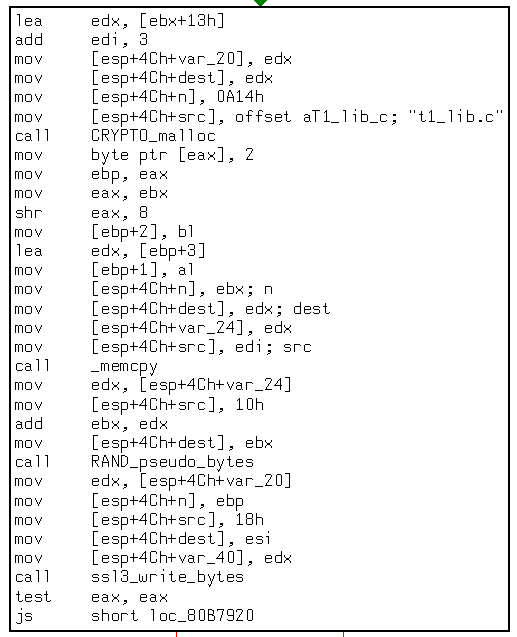
\includegraphics[height=4cm]{srj-figures/srj-gcc.png}
  \end{minipage}
  \begin{minipage}{.3\textwidth}

   \centering
  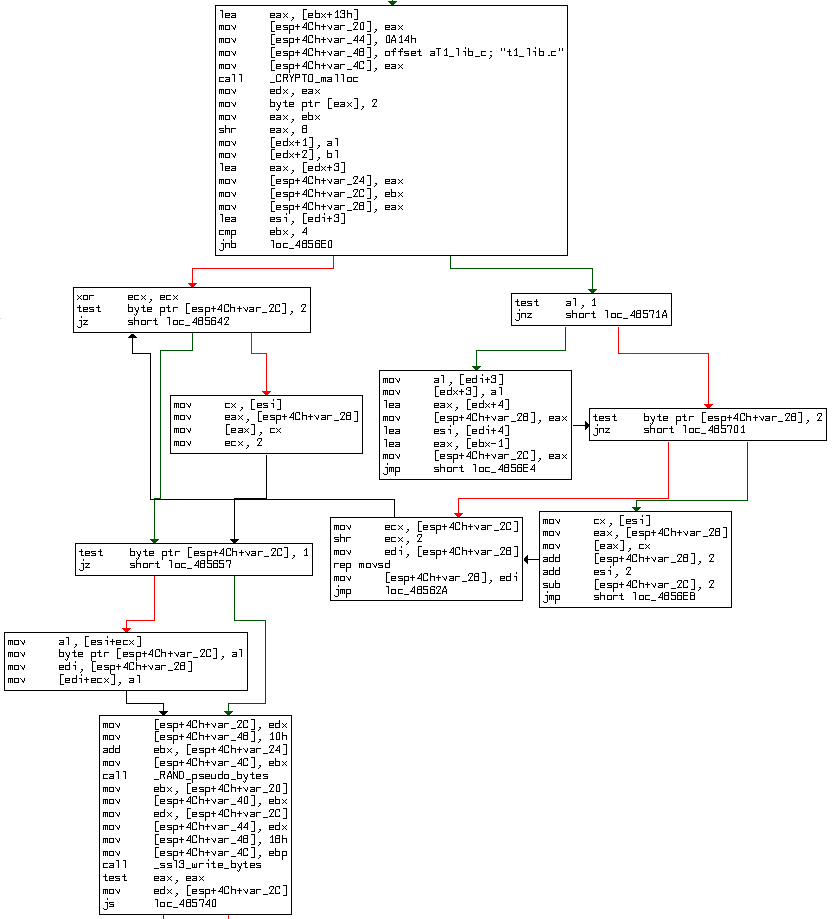
\includegraphics[height=6cm]{srj-figures/srj-mingw32.png}
     (c)
   \end{minipage}
  \caption{SSL/Heartbleed vulnerability (CVE-2014-0160) appeared as in the (a) actual source code, (b) binary compiled with GCC 4.6 for Linux OS, and (c) binary compiled with Mingw32 for Windows OS} \label{fig:prob_stat}
\end{figure*}

 \section{The system architecture of \tool}
\begin{figure*}[!ht]
	\centering
	%\includegraphics[width=1.0\textwidth]{srj-figures/srj-archi_new.pdf} %srj-archi
    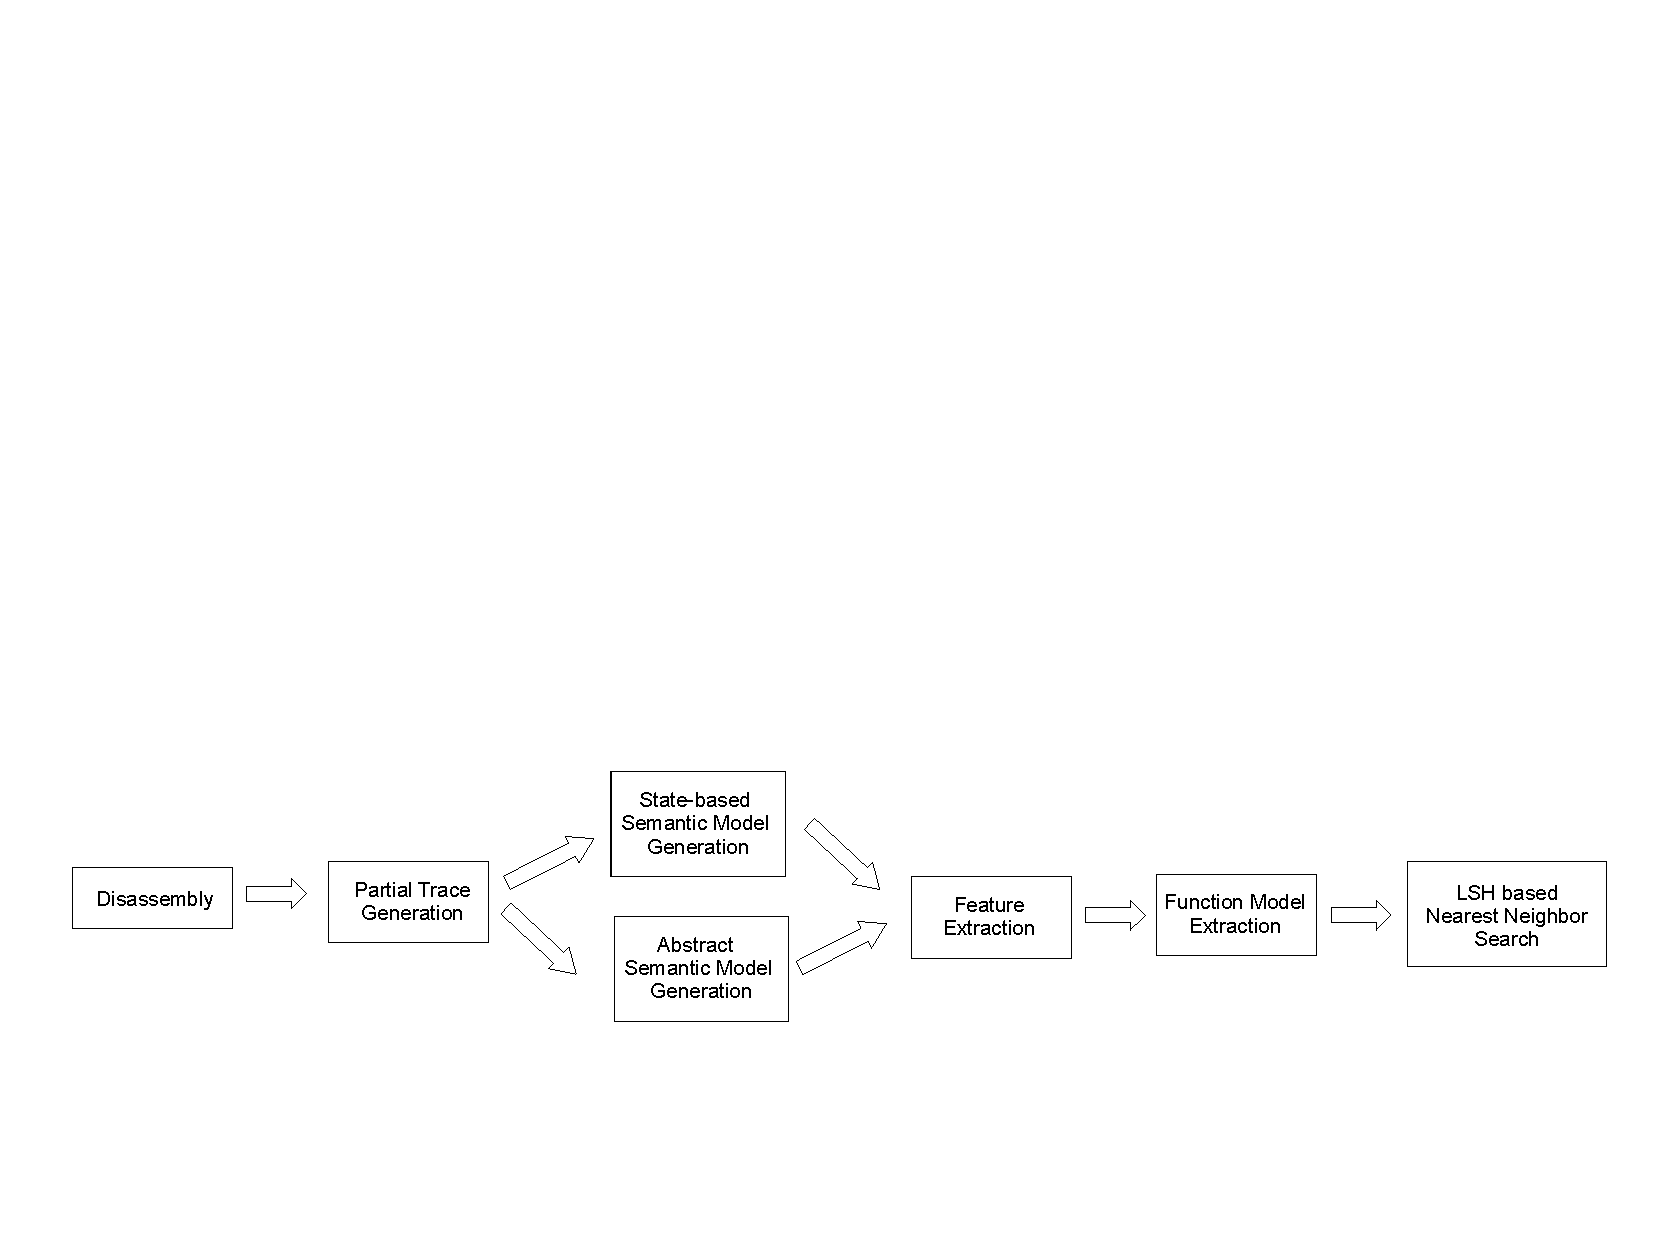
\includegraphics[width=1.0\textwidth]{srj-figures/srj-archi.pdf} %srj-archi
	\caption{\tool: Overview of system architecture}\label{fig:sys_arch}
\end{figure*}

\newpage
 \section{More Supporting experimental data} \label{app: exp_data2}

\begin{table*}[!ht]
	\begin{center}
		\caption{Rank distribution of matched functions \textbf{with} abstract structural, in \texttt{coreutils} binaries, across architectures (ARM, x86-32 and x86-64). We present the individual ranks for largest 14 binaries and at the end present the average of all other binaries \\}
		\label{tab:cross-arch-with-behav}
		\scriptsize
\begin{tabular}{ | l | l | l | l | l | l | l | l | l | l | l | l | l | }
\hline
	Binary & \multicolumn{2}{c|}{arm-gcc\_32} & \multicolumn{2}{c|}{arm-gcc\_64}  & \multicolumn{2}{c|}{gcc\_32-arm}  & \multicolumn{2}{c|}{gcc\_32-gcc\_64} & \multicolumn{2}{c|}{gcc\_64-arm}  & \multicolumn{2}{c|}{gcc\_64-gcc\_32}  \\ \hline
	 & Rank 1 & Top 5 & Rank 1 & Top 5 & Rank 1 & Top 5 & Rank 1 & Top 5 & Rank 1 & Top 5 & Rank 1 & Top 5 \\ \hline
	cp & 0.165 & 0.737 & 0.108 & 0.849 & 0.067 & 0.428 & 0.092 & 0.602 & 0.253 & 0.758 & 0.233 & 0.791 \\ \hline
	df & 0.176 & 0.696 & 0.155 & 0.831 & 0.041 & 0.405 & 0.126 & 0.599 & 0.268 & 0.739 & 0.287 & 0.749 \\ \hline
	dir & 0.114 & 0.653 & 0.064 & 0.771 & 0.052 & 0.342 & 0.103 & 0.532 & 0.181 & 0.739 & 0.246 & 0.837 \\ \hline
	du & 0.163 & 0.705 & 0.173 & 0.855 & 0.047 & 0.384 & 0.101 & 0.576 & 0.246 & 0.676 & 0.247 & 0.697 \\ \hline
	factor & 0.208 & 0.733 & 0.316 & 0.816 & 0.099 & 0.446 & 0.216 & 0.631 & 0.388 & 0.908 & 0.387 & 0.892 \\ \hline
	ls & 0.114 & 0.653 & 0.064 & 0.771 & 0.052 & 0.342 & 0.103 & 0.532 & 0.181 & 0.739 & 0.246 & 0.837 \\ \hline
	mv & 0.165 & 0.7 & 0.094 & 0.817 & 0.055 & 0.415 & 0.079 & 0.544 & 0.262 & 0.749 & 0.233 & 0.726 \\ \hline
	od & 0.168 & 0.674 & 0.198 & 0.78 & 0.074 & 0.4 & 0.157 & 0.639 & 0.264 & 0.901 & 0.389 & 0.88 \\ \hline
	sort & 0.153 & 0.729 & 0.092 & 0.815 & 0.085 & 0.475 & 0.105 & 0.665 & 0.225 & 0.763 & 0.205 & 0.755 \\ \hline
	split & 0.198 & 0.813 & 0.283 & 0.967 & 0.063 & 0.448 & 0.157 & 0.735 & 0.261 & 0.826 & 0.373 & 0.922 \\ \hline
	stat & 0.182 & 0.768 & 0.245 & 0.936 & 0.071 & 0.495 & 0.183 & 0.67 & 0.277 & 0.872 & 0.339 & 0.862 \\ \hline
	stdbuf & 0.184 & 0.816 & 0.386 & 0.976 & 0.103 & 0.494 & 0.242 & 0.737 & 0.349 & 0.952 & 0.394 & 0.909 \\ \hline
	tail & 0.179 & 0.813 & 0.13 & 0.917 & 0.045 & 0.5 & 0.115 & 0.68 & 0.25 & 0.815 & 0.287 & 0.836 \\ \hline
	vdir & 0.114 & 0.653 & 0.064 & 0.771 & 0.052 & 0.342 & 0.103 & 0.532 & 0.181 & 0.739 & 0.246 & 0.837 \\ \hline
	\textbf{Avg. large} & 0.163 & 0.725 & 0.169 & 0.848 & 0.065 & 0.423 & 0.134 & 0.620 & 0.256 & 0.798 & 0.294 & 0.824 \\ \hline
	\  & \  & \  & \  & \  & \  & \  & \  & \  & \  & \  & \  & \  \\ \hline
	\textbf{Avg. all other} & 0.273 & 0.889 & 0.3622 & 0.973 & 0.099 & 0.608 & 0.260 & 0.762 & 0.367 & 0.762 & 0.466 & 0.919 \\ \hline

\end{tabular}
\end{center}
\end{table*}


%Tabkle 13
\begin{table*}[!ht]
	\begin{center}
		\caption{Rank distribution of matched functions \textbf{without} abstract structural similarity, in \texttt{coreutils} binaries, across architectures (ARM, x86-32 and x86-64). We present the individual ranks for largest 14 binaries and at the end present the average of all other binaries \\}
		\label{tab:cross-arch-no-behav}
		\scriptsize

\begin{tabular}{ | l | l | l | l | l | l | l | l | l | l | l | l | l | }
\hline
		Binary & \multicolumn{2}{c|}{arm-gcc\_32} & \multicolumn{2}{c|}{arm-gcc\_64}  & \multicolumn{2}{c|}{gcc\_32-arm}  & \multicolumn{2}{c|}{gcc\_32-gcc\_64} & \multicolumn{2}{c|}{gcc\_64-arm}  & \multicolumn{2}{c|}{gcc\_64-gcc\_32}  \\ \hline
	 & Rank 1 & Top 5 & Rank 1 & Top 5 & Rank 1 & Top 5 & Rank 1 & Top 5 & Rank 1 & Top 5 & Rank 1 & Top 5 \\ \hline
	cp & 0.121 & 0.618 & 0.072 & 0.758 & 0.052 & 0.335 & 0.085 & 0.539 & 0.144 & 0.595 & 0.149 & 0.546 \\ \hline
	df & 0.096 & 0.622 & 0.034 & 0.746 & 0.03 & 0.333 & 0.086 & 0.586 & 0.136 & 0.568 & 0.164 & 0.569 \\ \hline
	dir & 0.075 & 0.532 & 0.039 & 0.732 & 0.023 & 0.266 & 0.066 & 0.636 & 0.087 & 0.52 & 0.149 & 0.554 \\ \hline
	du & 0.111 & 0.614 & 0.069 & 0.694 & 0.018 & 0.298 & 0.065 & 0.435 & 0.111 & 0.5 & 0.109 & 0.471 \\ \hline
	factor & 0.09 & 0.652 & 0.08 & 0.773 & 0.045 & 0.303 & 0.125 & 0.639 & 0.133 & 0.653 & 0.153 & 0.611 \\ \hline
	ls & 0.075 & 0.532 & 0.039 & 0.732 & 0.023 & 0.266 & 0.066 & 0.636 & 0.087 & 0.52 & 0.149 & 0.554 \\ \hline
	mv & 0.134 & 0.603 & 0.096 & 0.692 & 0.045 & 0.346 & 0.054 & 0.497 & 0.16 & 0.577 & 0.15 & 0.51 \\ \hline
	od & 0.083 & 0.583 & 0.066 & 0.658 & 0.048 & 0.298 & 0.067 & 0.627 & 0.105 & 0.763 & 0.133 & 0.707 \\ \hline
	sort & 0.117 & 0.58 & 0.05 & 0.693 & 0.056 & 0.352 & 0.055 & 0.579 & 0.107 & 0.521 & 0.097 & 0.503 \\ \hline
	split & 0.094 & 0.647 & 0.066 & 0.842 & 0.035 & 0.306 & 0.116 & 0.725 & 0.118 & 0.632 & 0.145 & 0.609 \\ \hline
	stat & 0.124 & 0.64 & 0.101 & 0.886 & 0.045 & 0.337 & 0.113 & 0.803 & 0.114 & 0.671 & 0.169 & 0.761 \\ \hline
	stdbuf & 0.104 & 0.701 & 0.045 & 0.881 & 0.065 & 0.39 & 0.143 & 0.857 & 0.134 & 0.761 & 0.206 & 0.714 \\ \hline
	tail & 0.131 & 0.697 & 0.081 & 0.791 & 0.03 & 0.364 & 0.073 & 0.756 & 0.116 & 0.593 & 0.122 & 0.646 \\ \hline
	vdir & 0.075 & 0.532 & 0.039 & 0.732 & 0.023 & 0.266 & 0.066 & 0.636 & 0.087 & 0.52 & 0.149 & 0.554 \\ \hline
	\textbf{Avg. large} & 0.102 & 0.611 & 0.0626 & 0.757 & 0.0384 & 0.318 & 0.0842 & 0.639 & 0.117 & 0.599 & 0.146 & 0.593 \\ \hline
	\  & \  & \  & \  & \  & \  & \  & \  & \  & \  & \  & \  & \  \\ \hline
	\textbf{Avg. all other} & 0.161 & 0.784 & 0.204 & 0.912 & 0.0589 & 0.460 & 0.160 & 0.899 & 0.157 & 0.791 & 0.194 & 0.811 \\ \hline
\end{tabular}
\end{center}
\end{table*}


\begin{table*}[!ht]
\begin{center}
\caption{Ranks obtained by \tool for functions in \texttt{msvcrt.dll} (closed-source) against \texttt{libc.so} (open-source). \\}
		\label{tab:msvcrt_libc}
		\scriptsize
%\begin{tabular}{ | l | l | l | l | l | }
\begin{tabular}{|m{0.8cm}|m{12cm}|m{0.7cm}|m{0.7cm}|m{0.7cm}|}
\hline
	Ranks & Matched functions & No. of Functions & \% & Cum. \% \\ \hline
	1 & \texttt{tolower, memset, wcschr, wcsncmp, toupper, memcmp, strspn, wcsrchr, memchr, log} & 10 & 15.6 &  15.6\\ \hline
	2-3 & \texttt{wcstoul, wcstol, strtoul, fopen, strncpy, strtol, itoa, wcscmp, wcsncat, itow, strrchr, strchr, longjmp, strcspn, wcsncpy, labs, strpbrk, toupper, write, memcpy, memmove, tolower, modf} & 23 & 35.9 & 51.6 \\ \hline
	4-5 & \texttt{mbtowc, wcstombs, strcat, remove, mbstowcs, wctomb} & 6 & 9.3 & 60.9 \\ \hline
	6-10 & \texttt{rename, strstr, wcspbrk, iswctype, strtok, wcscoll, strcoll, setlocale, qsort, wcsspn, swprintf, wcstod, strerrorr} & 13 & 2.3 &  81.3\\ \hline
	11-20 & \texttt{strncat, raise, strtod, wcscspn, wcstok, atol} & 6 & 9.3 &  90.6\\ \hline
	21-50 & \texttt{ldexp, perror, system, wcsxfrm} & 4 & 6.3 & 96.9 \\ \hline
	51-100 & \texttt{frexp, strxfrm} & 2 & 3.1 & 100.0 \\ \hline
\end{tabular}
\end{center}
\end{table*}

 %change to double column


\end{appendices}


